%=========================
% Materials and Methods
%=========================

% Your not including yield in your analysis? Seems to be a big reason for this work. Why is it not included?
This research will use data collected from surveys of irrigated lowland rice growing areas in South and South East Asia to examine relationships between the injuries caused by pests and diseases, cropping practices (\textit{e.g.}, rice variety grown, crop establishment method, fertilizer and chemicals applied). Their relationships will be constructed and analyzed through network analysis. I will develop and apply suitable methods of network analysis to characterize the associations of injuries and cropping practices. The resulting network of associations of injuries and cropping practices will thus provide a starting point for further investigations of their relationships (\textit{i.e.}, characterization of relationships of cropping practices and injury profiles related to yields, comparison of networks under different production environments or examination of networks at different levels of yield gains). 

In the following, I present three distinct network analysis approaches: single-network analysis, differential network analysis, and dynamic network analysis. These three approaches will answer different questions. I will apply single-network analysis to the data from all fields surveyed for identifying patterns of interactions between injuries and cropping practices and key components (\textit{e.g.}, most connected variables). Second, differential network analysis will aim to uncover similarities and differences of networks constructed from the different data sets (\textit{e.g.}, dry season versus wet season). Dynamic network analysis, the third type, will be applied to study how networks changed under at least two different aspects of an evolving complex system. Here, I will focus on dynamic networks by dividing farms into different levels of yield attained. 

\subsection*{Crop health survey data}
\addcontentsline{toc}{subsection}{Crop health survey data}

% how many farmers' fields were surveyed?
Crop health survey data were collected through surveys of farmers' fields (approximately 800) from 2010 to 2015 for both wet and dry seasons in different production environments across South and South East Asia representing irrigated lowland rice growing areas West Java, Indonesia; Mekong River Delta and Red River Delta, Vietnam; Tamil Nadu and Odisha, India; and Suphanburi, Thailand. The survey protocol described in the IRRI publication, ``A SURVEY PORTFOLIO TO CHARACTERIZE YIELD-REDUCING FACTORS IN RICE'', \citep{Savarysurvey2009} was used for data collection. The variables collected included environmental attributes, patterns of cropping practices, crop growth measurement and crop management status assessments, measurements of levels of injuries caused by pests, and direct measurements of actual yields from crop cuts. The data collected can be classified into three groups: cropping practices, injuries, and actual yield measurements.

Cropping practice data included information on the type of rice variety (traditional variety, modern variety, or hybrid rice), crop establishment methods used (direct seeded or transplanted rice) and were collected as categorical data. Pesticide usage (molluscicide, herbicide, insecticide and fungicide) were collected as discretized data, and accumulated organic, synthetic fertilizers were collected as continuous data.

Injury data were gathered on diseases, insects and weeds observed at two development stages of the growing crop: active tillering and active ripening. While injuries due to diseases and insects were specific to species (or species groups), information on weed infestation was the area covered by any weed species, either above or below the crop canopy. Information pertaining to injuries was collected in the form of number of injured organs (tillers, leaves, and panicles), which later was made relative to the corresponding total number of organs present in the sampling units; 12 hills per field for transplanted rice crops, or 12 $\times$ 10 cm quadrat for direct seeded rice. As for weed infestation, the proportion of soil area covered at two levels of the crop canopy (below or above) was assessed in three points in the field of 1 $mathrm{m}^{2}$ each. For this purpose, two types of injury indices were used: area under injury progress curves (AUIPC) or maximum level at any of the two observations, depending on the nature of the injury. Injuries which is occurred on tillers, hills and panicles were quantified as maximum level, whereas juries which occurred on leaf were quantified as AUIPC. The AUIPC was calculated by the mid- point method using the following equation: $\mathrm{AUIPC} = \sum\limits_{i=1}^n\frac{1}{(x_{i} + x_{i-1})(T_{i} - T_{i-1})}$, where $x_i$ is percentage (\%) of leaves, tillers or panicles injured caused by pests (e.g., leaf blast, leaf folder), percentage (\%) of weed infestation (ground coverage) at the \textit{i}th observation, $\mathrm{T}_{i}$ is time in rice development stage units (DSU) on a 0 to 100 scale (10: seedling, 20: tillering, 30: stem elongation, 40: booting, 50: heading, 60: flowering, 70: milk, 80: dough, 90: ripening, 100: fully mature) at the $i$th observation where $n$ is total number of observations.

% Corrected for tense.
% yield data weren't "estimated" they were measured.
% corrected for clarity.
Yield data were measured from three randomly selected crop cuts that were 5 $\mathrm{m}^{2}$ (2 $\times$ 2.5 meters) and dried to 14\% moisture content and weighed.

\section*{Single network analysis of crop health survey data}
\addcontentsline{toc}{section}{Single network analysis of crop health survey data}

%% 1. First sentence is unclear.
Cropping practices and injury profiles network will be constructed from the pair--wise correlation matrix between any variables of injuries (insect injuries and diseases) and cropping practices (fertilizer usage, pesticide applied,rice varieties and crop establishment methods). The edges of the network will correspond to the degree of correlation between two variables. A standard measurement of correlation between two variable $x$ and $y$, $cor(x,y)$, where values are  between -1 to +1 depending on the level of relationship. $cor(x_{i}, x_{j})$ is equal to -1 when there is a decreasing relationship between $x$ and $y$, and +1 when there is a increasing relationship.

To identify the most suitable pairwise correlation methods, I will evaluate four correlation based measures, Pearson's correlation, Spearman's rank correlation, Kendall's correlation, and biweight midcorrealtion. The statistical programming language \textsf{R} will be employed to compute pairwise correlation \citep{R:2014a}. The \texttt{cor.test()} function will be applied for generating a correlation matrix, which describes the pairwise correlations between variables. This function allows users to choose types of correlation measures to perform such as Pearson's correlation, Spearman's rank correlation and Kendall's rank correlation. To compute biweight midcorrelation, I will apply the \texttt{bicor()} function from the \textbf{WGCNA} package \citep{Langfelder:2008bd} in \textsf{R}. 

% p-values should be determined or calculated?
When a correlation matrix is created, the next step is to construct the correlation based network. However, $p$~values should be determined because correlation will be considered if    its $p$~value is less than $p$~values at considered significant (\textit{e.g.}, 0.01, 0.05). As with issues previously mentioned above, $p$~values must be adjusted for multiple testing. Using a Benjamini-Hochberg adjustment or Bonferonni correction is recommended by \citet{kolaczyk2014statistical}. The \texttt{fdrtool()} function of \textbf{fdrtool} R package can calculate adjusted $p$~values. These values are compared to a standard 0.05 significance level. The final correlation matrix contains pair-wise correlation coefficients, which have adjusted for $p$~values lower than 0.05 significance level.

% 1. The first sentence after that is still unclear.
The \textsf{R} packages: \textbf{igraph} \citep{Csardi:2010wx}; \textbf{qgraph} \citep{qgraph}; \textbf{statnet} \citep{statnetpackage} and \textbf{network} \citep{networkpackage}; and \textbf{sna} \citep{snapackage} will be used to construct and analyze network models.

%====================== Comments===================
% why knowledge of biological literature? Why not a good understanding of the biological system that you are monitoring? I think that's more essential and useful
% models cannot reveal knowledge, look up the definition of knowledge. It does not apply here. What do you really mean because it can not be knowledge?
% first sentence, all of them what?
% based on what study? Our study? Who is "we"? This is YOUR research. If anything it should be "based on my study" but I'm not clear as to what study you refer to here. Who are the "we" that are suggesting? You're the only author on this manuscript. It's your dissertation. There is no, our, us or we. It's only my, me, I here.
% Is "codes" the proper form to use?

\subsection*{Evaluating network properties}

% Last sentence, WHAT biological properties interest you?
Once a network is constructed, several indices will be computed to convey information about network structure. To evaluate the topological properties of both the interaction and the correlation based network, I will use the packages \textbf{igraph} and \textbf{qgraph} in \textsf{R} \citep{qgraph}. I am particularly interested in properties potentially relevant for biological roles and functioning as previously hypothesized in other biological networks \citep{Strogatz:2001wc, horvath2011weighted}. For example, connected hub nodes are focused because they have high connectivity, which mean they have relationships with many nodes. In the following, there are some network indices used to describe the topological properties of single network and for comparing two or more networks (\textit{e.g}. , differential , and dynamic network analysis) 

% This comment is unaddressed? What is this section? You need some sort of introduction to this list of items. Are these the items of interest? If so you need a lead in as I said, you need an introduction to this. It's just abrupt. Suddenly there's a list. It does not flow.

\begin{enumerate}
\item Mean degree: the degree of a node counts the number of edges it has. The mean degree is calculated over all nodes in the network.
\item Degree distribution: the frequency of nodes vs. their (increasing) degree.
\item Average shortest path length: the shortest path between any two nodes is the single path with fewest edges between them. Alternative paths are feasible. The average shortest path length is the mean over all shortest paths between any two nodes in the network.
\item Mean clustering coefficient: a cluster of nodes is a triangle of nodes. The clustering coefficient calculates the fraction of observed vs. possible triangles for each node. The mean is subsequently determined from all nodes in the network.
\item Betweenness centrality: the betweenness centrality of a node is equal to the number of shortest paths between any two nodes in the graph passing through that node. The mean is calculated from all nodes in the network.
\item Closeness centrality: the closeness centrality of a node is given by the average distance of this node to any other node. Again, the network-wide measure is an average over all nodes in the network.
\end{enumerate}

\citet{Deng:2012do, Toubiana:2013cv, horvath2011weighted, newman2003structure} are recommended references for descriptions of the network properties as well as the formal calculation of these measures.

%====================================================
\section*{Differential network analysis of crop heath survey data}

\addcontentsline{toc}{section}{Differential network analysis of crop health survey data}

% methods
% This isn't normal English, "With in my focuses, they will be produced from  adjacency metrics,"
Differential networks will be constructed from the survey data with different groups of samples. With in my focuses, they will be produced from adjacency metrics, which are encoded with correlation coefficients of any variables under different conditions (dry and wet season). To analyze differential networks in different seasons, I will determine the differential relationships of any variables in cropping practices and injuries between dry season network and wet season network. Additionally I will construct differential networks under different production environments (locations).

For comparison with a standard differential network analysis, I will use the \textbf{WGCNA} \citep{horvath2011weighted} and \textbf{dna} \citep{dnapackage} packages in \textsf{R}. These packages provide several functions to analyze the different structures of two networks \citep{horvath2011weighted}. These functions include preprocessing tools for simultaneously preparing a pair of networks for analysis, procedures for computing connectivity scores between pairs of variables based on many available statistical techniques, and tools for handling modules of variables based on these scores. Also, procedures are provided for performing permutation tests based on these scores to determine if the connectivity of variables differs between the two networks, to determine if the connectivity of a particular set of important variables differs between the two networks, and to determine if the overall module structure differs between the two networks. Several built-in options are available for the types of scores and distances used in the testing procedures, and additionally, the procedures provide flexible methods that allow the user to define custom scores and distances. For example, the \texttt{test.modular.structure()} function is used to compare between the connectivity measures of each network \citep{dnapackage}.
 
\section*{Dynamic network analysis of crop health survey data}
\addcontentsline{toc}{section}{Dynamic network analysis of crop health survey data} 

Dynamic network analysis will be applied to study changes in networks with at least two different aspects of an evolving complex system. Dynamic networks of crop health survey data at three different levels of farmers' yields will be constructed. Surveys contain records of observed actual yields, various types of injuries and cropping practices. To generate the data set for constructing the dynamic network, I will group the data with successive levels of yields to obtain different yield data sets in order to construct a dynamic network of yield-varying behaviors. I then will employ \textbf{networkDynamic} \citep{networkdynamicpackage} and \textbf{ndtv} \citep{ndtvpackage} packages to generate yield-varying networks. The dynamic graphs will be characterized following \citep{bilgin2006dynamic, kolaczyk2014statistical}. From the network based perspectives, the results will show the patterns of interactions between nodes how they changed when levels of yield decreased or increased.

%\begin{landscape}
\begin{figure}
\centering
%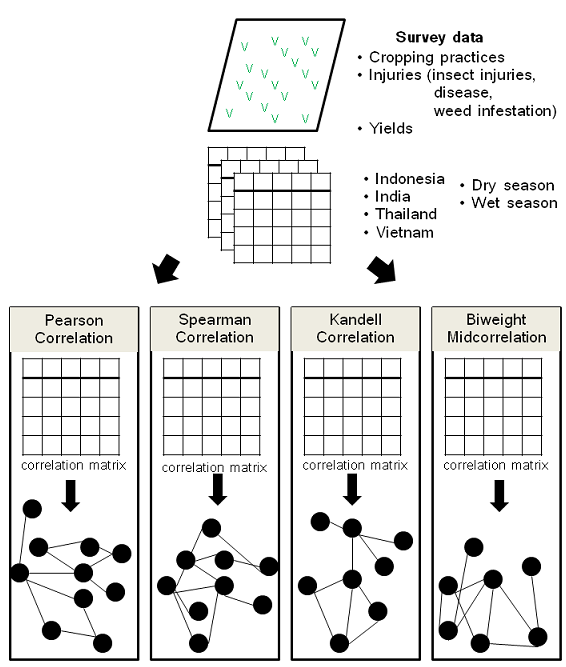
\includegraphics[resolution = 600]{pipeline}
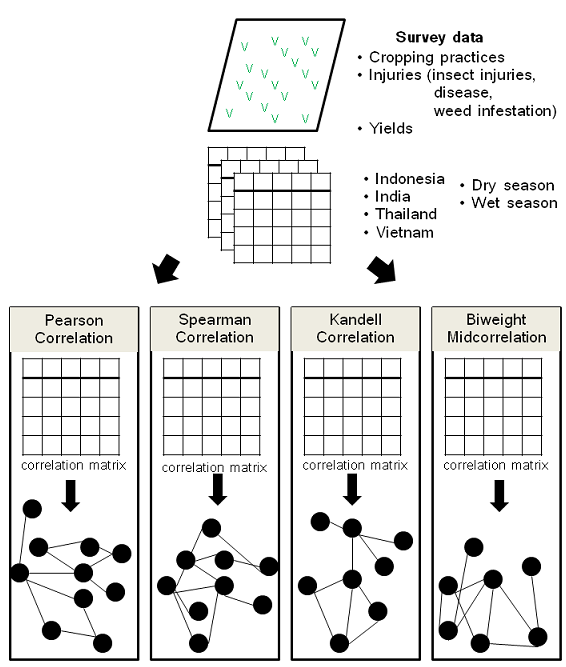
\includegraphics[width = 6in]{pipeline}
% What is FDR correction? A caption should enable a figure to stand on its own.
\caption[Network method for characterizing interactions between injury profiles and cropping practices using correlation measures]{Crop health survey data that were collected include cropping practices, injuries, and yield data. These data were collected from farmers' fields in four countries: Indonesia, India, Thailand, and Vietnam. Correlation matrices will be produced using four individual methods; Pearson, Spearman, Kendall correlation and Biweight midcorrelation. The $p$~values for all coefficients will be adjusted by FDR correction. The correlation coefficients with $p$~values > 0.05 will be removed. The resulting network will be analyzed for structural properties and to infer biological meanings. This will provide the cropping practices and injury profiles network of crop health data.}
\end{figure}
%\end{landscape}

\newpage
\begin{landscape}
\begin{figure}
\centering
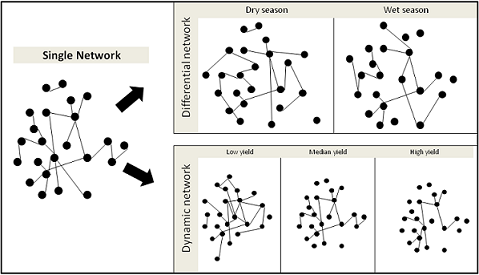
\includegraphics[width=8in]{wholenet}
\caption[Network comparison]{A single network will be created from the whole survey data set. Differential networks will be constructed using different data set, which may be different subgroups of samples from different seasons (\textit{e.g.}, dry season and wet season) or different geographic locations, then differences in connectivity patterns between two networks will be measured. Dynamic networks will be produced from different subgroups of surveys by grouping consecutive yield levels, (\textit{i.e.}, low, median, high yield).}
\end{figure}
\end{landscape}

%================eos================================